\section{实验}\label{experiment}
我们将 \computerrl 应用于 \glm~\citep{glm2024chatglm}与 \glmv~\citep{hong2025glm}，得到 \model-9B。
我们在多种场景下开展广泛实验，以评估 \model 在计算机环境中的性能。

\begin{table*}[t!]
\centering
\caption{\model 在 OSWorld 与 OSWorld-Verified 上的性能（更新于 2025 年 8 月）。我们将 \model 与包括专有模型和开放模型在内的最先进智能体进行比较。}
\vspace{-3mm}
\renewcommand\tabcolsep{8pt}
\label{tab:osworld}
\resizebox{\columnwidth}{!}{
\begin{tabular}{@{}p{7.5cm}ccc@{}}
\specialrule{1.0pt}{1.0pt}{1.0pt}
\textbf{智能体模型} & \textbf{参数量} & \textbf{OSWorld} & \textbf{OSWorld-Verified} \\
\specialrule{1.0pt}{1.0pt}{1.0pt}
\multicolumn{4}{@{}l}{\textit{专有模型}} \\
Aria-UI w/ GPT-4o~\citep{yang2024aria} & - & 15.2 & - \\
Aguvis-72B w/ GPT-4o~\citep{xu2024aguvis} & - & 17.0 & - \\
Claude 3.7 Sonnet~\citep{claude2} & - & 28.0 & 35.8 \\
Claude 4.0 Sonnet~\citep{claude2} & - & 30.7 & 43.9 \\
Agent S2 w/ Claude-3.7-Sonnet~\citep{agashe2025agent} & - & 34.5 & - \\
InfantAgent~\citep{lei2024infant} & - & 35.3 & - \\
OpenAI CUA 4o~\citep{cua2025} & - & 38.1 & 31.3 \\
Agent S2 w/ Gemini-2.5-Pro~\citep{agashe2025agent} & - & 41.4 & 45.8 \\
UI-TARS-1.5~\citep{qin2025ui} & - & 42.5 & - \\
OpenAI CUA o3~\citep{cua2025} & - & 42.9 & - \\
\midrule[\heavyrulewidth]
\multicolumn{4}{@{}l}{\textit{开放模型}} \\
Qwen2.5-vl-72B~\citep{bai2023qwen-vl} & 72B & 8.8 & 5.0 \\
PC Agent-E~\citep{he2025efficient} & 72B & 14.9 & - \\
UI-TARS-72B-SFT~\citep{qin2025ui} & 72B & 18.8 & - \\
UI-TARS-72B-DPO~\citep{qin2025ui} & 72B & 24.6 & 27.1 \\
UI-TARS-1.5-7B~\citep{qin2025ui} & 7B & 26.9 & 27.4 \\
Jedi-7B w/ GPT-4o~\citep{xie2025scaling} & ~~7B+ & 27.0 & 29.3 \\
UI-TARS-7B-1.5 + ARPO~\citep{lu2025arpo} & 7B & 29.9 & - \\
\midrule[\heavyrulewidth]
\multicolumn{4}{@{}l}{\computerrl \textit{（本文）}} \\
\quad w/ \glm & 9B & \underline{48.1$\pm$1.0} & \underline{47.3} \\
\quad w/ \glmv & 9B & \textbf{48.9$\pm$0.5} & \textbf{48.0} \\
\specialrule{1.0pt}{1.0pt}{1.0pt}
\end{tabular}
}
\end{table*}


\subsection{主要结果}\label{exp:osworld}
为了更贴近真实用户体验，我们在 OSWorld~\citep{xie2024osworld}和\href{https://xlang.ai/blog/osworld-verified}{OSWorld-Verified} 基准上评估 \model，并将其性能与 CUA~\citep{cua2025}、Claude-4~\citep{claude2}和 UI-TARS~\citep{qin2025ui}等最先进模型进行比较。比较结果见表~\ref{tab:osworld}。
结果表明，\model 在多个领域均取得了更优性能，其中优势在具有挑战性的多应用设置中最为明显。此外，借助 API-GUI 策略，\model 最多只需最强基线方法所用步骤的 \textbf{1/3} 即可完成任务，展现出显著的执行效率提升。这些结果凸显了 \computerrl 在多种应用中推进计算机自动化技术前沿的潜力。

\subsection{办公应用性能}
办公应用是交付与展示工作成果的关键界面，因此构成了评估计算机使用智能体的重要测试平台。
为了评估智能体在该领域的性能，我们从三个来源精选了 180 项具有挑战性的任务：SpreadsheetBench~\citep{ma2024spreadsheetbench}、PPTC~\citep{guo2023pptc}，以及我们内部开发的 Writer 领域任务。我们根据需要对这些任务进行适配，使其能够集成到 OSWorld 框架中。得到的基准称为 \textbf{OfficeWorld}，可用于系统衡量智能体在办公场景中的能力。结果见表~\ref{tab:officeworld}。

\begin{table*}[h!]
\centering
\caption{\model 在 OfficeWorld 上与常用基线相比的性能。我们采用相同的框架（含工具）与测试设置，以保证比较公平。}
\vspace{-3mm}
\renewcommand\tabcolsep{12pt}
\label{tab:officeworld}
\resizebox{\columnwidth}{!}{
\begin{tabular}{@{}p{7.5cm}cccc@{}}
\specialrule{1.0pt}{1.0pt}{1.0pt}
\textbf{智能体模型} & \textbf{Word} & \textbf{Excel} & \textbf{PPT} & \textbf{平均值} \\
\specialrule{1.0pt}{1.0pt}{1.0pt}
DeepSeek-V3.1~\citep{liu2024deepseek} & 6.7 & 35.0 & 21.7 & 21.1 \\
DeepSeek-R1~\cite{guo2025deepseek} & 13.3 & 36.7 & 18.3 & 22.8 \\
Claude 3.7 Sonnet~\citep{claude2} & 15.0 & 25.0 & 25.0 & 21.7 \\
Claude 4.0 Sonnet~\citep{claude2} & 18.3 & 35.0 & 20.0 & 24.4 \\
Gemini-2.5-Pro~\citep{team2023gemini} & 5.0 & 11.7 & 20.0 & 12.2 \\
GPT-4o~\citep{hurst2024gpt} & 18.3 & 21.7 & 8.3 & 16.1 \\
GPT-4.1~\citep{achiam2023gpt} & 21.7 & 25.0 & 28.3 & 25.0 \\
OpenAI o3~\citep{jaech2024openai} & \underline{23.3} & 36.7 & \underline{41.7} & 33.9 \\
\midrule[\heavyrulewidth]
\multicolumn{5}{@{}l}{\computerrl \textit{（本文）}} \\
\quad w/ \glm & 21.7 & \textbf{58.3} & \textbf{43.3} & \underline{41.1} \\
\quad w/ \glmv & \textbf{30.0} & \textbf{58.3} & \underline{41.7} & \textbf{43.3} \\
\specialrule{1.0pt}{1.0pt}{1.0pt}
\end{tabular}
}
\end{table*}


\subsection{消融研究}
为了评估不同算法与训练数据集对智能体性能的影响，我们在表~\ref{tab:ablation_study}中给出了 OSWorld 基准上的消融研究。

\begin{table}[t]
\caption{框架设计与训练方法的消融研究。我们将 OSWorld 划分为五个不同领域，以便更细致地比较不同策略在各领域中的效果。}
\vspace{-2mm}
\label{tab:ablation_study}
\centering
\renewcommand\tabcolsep{12pt}
\resizebox{\columnwidth}{!}{
\begin{tabular}{@{}lcccccc@{}}
\toprule
方法 & OS & Office & Daily & Professional & Workflow & 平均值 \\
\midrule
\multicolumn{7}{c}{框架消融（使用 \gptfouro）}\\
\midrule
仅 GUI & 41.7 & 6.2 & 12.3 & 14.3 & 7.5 & 11.2 \\
API-GUI & 52.6 & 27.9 & 25.7 & 41.6 & 10.8 & 26.2 \\
\midrule
\multicolumn{7}{c}{训练消融}\\
\midrule
未训练 & 20.8 & 17.2 & 19.7 & 22.9 & 3.3 & 15.2 \\
$+$ 行为克隆 & 54.2 & 35.0 & 37.2 & 45.8 & 10.8 & 31.9 \\
$+$ RL 阶段 1 & 83.3 & 46.1 & 45.1 & 56.3 & 16.1 & 42.0 \\
$+$ \rlmethod & 75.0 & 42.3 & 50.6 & 52.1 & 18.9 & 41.5 \\
$+$ RL 阶段 2 & \textbf{83.3} & \textbf{46.2} & \textbf{46.7} & \textbf{60.4} & \textbf{27.2} & \textbf{45.8} \\
\bottomrule
\end{tabular}
}
\end{table}


\vpara{框架消融。}
我们使用 \gptfouro，对仅使用 GUI 的方法与所提出的 API-GUI 范式进行性能比较。结果表明，API-GUI 范式在所有领域都大幅优于仅使用 GUI 的基线。具体而言，API-GUI 策略的平均成功率达到 26.2\%，相较仅使用 GUI 的方法（11.2\%）提升了 134\%。最显著的增益出现在 Office 领域（27.9\% 对 6.2\%）和 Professional 领域（41.6\% 对 14.3\%），API-GUI 分别带来 350\% 和 191\% 的提升。这些结果验证了我们的核心假设：将 API 调用与 GUI 交互结合，可以更高效、更可靠地执行任务，尤其适用于能够受益于程序化控制的复杂专业工作流。

\begin{figure}[t]
    \centering
    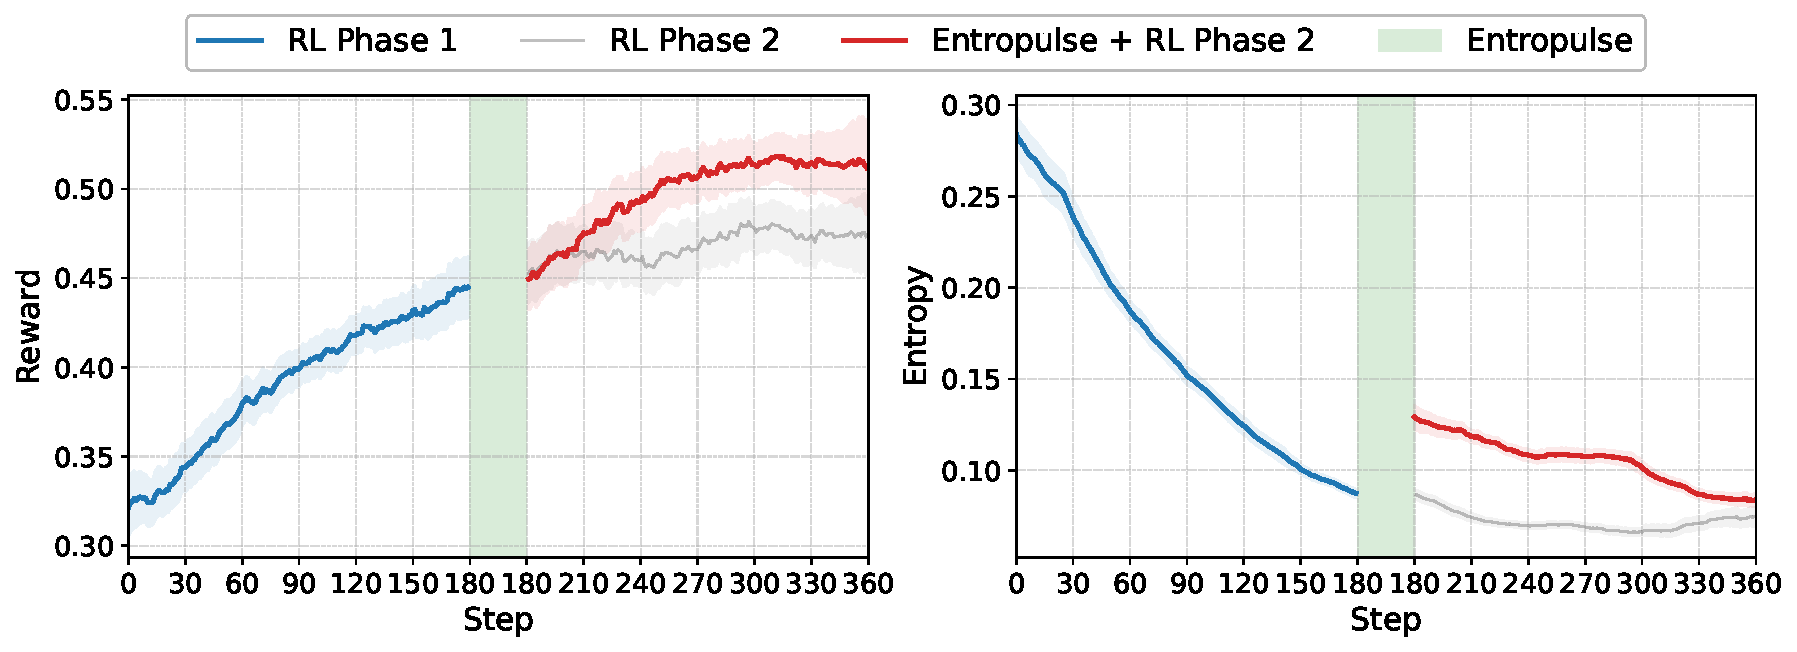
\includegraphics[width=\linewidth]{images/rl_curve_reward_entropy_exp.pdf}
    \vspace{-7mm}
    \caption{\computerrl 的训练奖励曲线（左）与熵曲线（右），阴影为 95\% 置信区间。红线表示在第一阶段 RL 后通过 \rlmethod 恢复熵的训练过程，灰线则表示仅重置参考模型后继续训练。}
    \label{figs:trending}
\end{figure}

\vpara{训练消融。}
我们使用 \qwen 研究不同训练阶段逐步产生的影响。
从骨干模型出发，行为克隆（BC）以 31.9\% 的性能奠定了坚实基础。第一阶段 RL（RL1）带来显著增益，使性能提升至 42.0\%（提高 10.1 个百分点）。
值得注意的是，\rlmethod 阶段在保持近似性能（41.5\%）的同时，显著提高了动作熵；这增强了探索多样性，使最终的 RL2 阶段能够进一步改进。
RL2 阶段达到 45.8\% 的最佳性能（相较 RL1 提高 3.8 个百分点），受益于 \rlmethod 所引入的更强探索能力。
值得一提的是，Workflow 领域在整个训练过程中提升最为显著（10.8\% $\rightarrow$ 27.2\%），其他领域则始终保持较高性能，这突出表明多阶段训练十分重要。

\vpara{RL 可扩展性。}
我们在图~\ref{figs:trending}中给出 RL 的训练奖励与熵曲线，以研究 \rlmethod 对延长 RL 训练动态的影响。
第一阶段 RL 收敛后，我们比较采用与不采用 \rlmethod 的第二阶段 RL。为保证比较公平，我们在两种设置中都重置参考模型。

结果表明，引入 \rlmethod 会提高模型的熵，从而恢复其探索能力。增强后的探索显著扩展了有效训练步数，并最终提升整体性能。

\subsection{案例研究与错误分析}

\begin{wrapfigure}[13]{r}{0.28\textwidth}
    \vspace{-13mm}
    \centering
    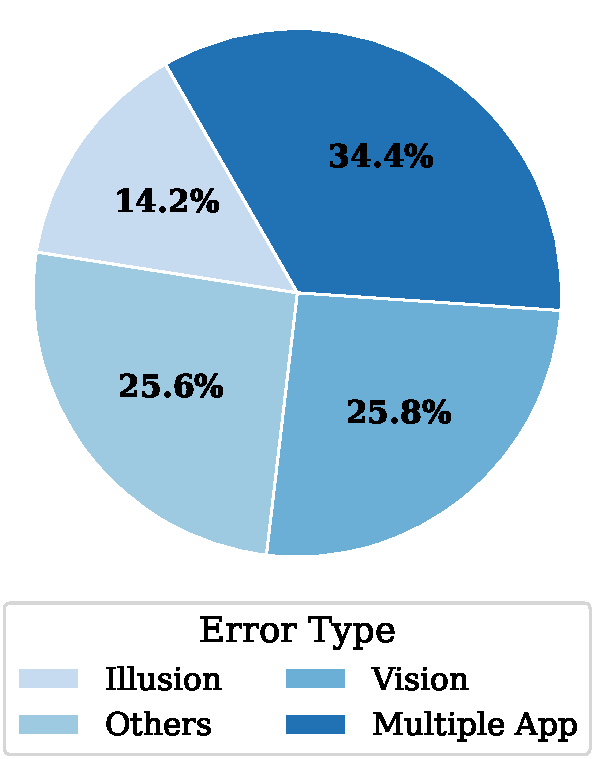
\includegraphics[width=0.9\linewidth]{images/error_analysis.pdf}
    \caption{错误分布。}
    \label{figs:error_analysis}
\end{wrapfigure}

我们在桌面环境中开展案例研究，以识别系统潜在的优化方向。尽管模型在大多数场景中表现稳健，我们仍发现了若干局限。具体而言，任务执行过程中遇到的错误可以分为四种主要类型：视觉感知错误、多应用协调失败、操作幻觉以及其他错误。这些错误类型的分布见图~\ref{figs:error_analysis}。

附录~\ref{apdx:demo}还给出了更多具有代表性的成功与失败案例，以进一步说明模型的能力与局限。
